\documentclass[12pt,a4paper]{article}

\usepackage[utf8]{inputenc}
\usepackage[polish]{babel}
\usepackage[T1]{fontenc}
\usepackage{amsmath}
\usepackage{amsfonts}
\usepackage{graphicx}
\usepackage{geometry}
\usepackage{hyperref}
\usepackage{float}
\usepackage{listings}
\usepackage{xcolor}
\usepackage{booktabs}
\usepackage{multirow}
\usepackage{subcaption}

\geometry{
    left=2.5cm,
    right=2.5cm,
    top=2.5cm,
    bottom=2.5cm
}

\graphicspath{{figures/}}

\lstset{
    basicstyle=\ttfamily\small,
    breaklines=true,
    frame=single,
    commentstyle=\color{gray},
    keywordstyle=\color{blue},
    stringstyle=\color{red}
}

\begin{document}

\begin{flushright}
Gliwice, \today
\end{flushright}

\vspace{1cm}

\begin{center}
{\Large \textbf{Modelowanie matematyczne}}\\[0.5cm]
{\Large Dokumentacja projektu końcowego}\\[1cm]

{\large \textbf{Tytuł:} Krzywa pogoni}\\[0.5cm]

{\large \textbf{Autorzy:} Skowroński Piotr, Czuba Krzysztof}\\[0.3cm]

{\large \textbf{Kierunek:} Informatyka, studia 2 stopnia (sem. II)}
\end{center}

\vspace{1cm}

\tableofcontents
\newpage

\section{Cel zadania}

Celem projektu jest implementacja i analiza różnych strategii pościgu  w przestrzeni euklidesowej oraz na rozmaitościach riemannowskich. Projekt obejmuje:

\begin{itemize}
    \item Implementacja klasycznych strategii pościgu w 2D: bezpośredniego pościgu, pościgu przy stałym namiarze, nawigacji proporcjonalnej oraz pościgu cyklicznego.
    \item Rozszerzenie strategii na przestrzeń 3D oraz ogólną przestrzeń n-wymiarową
    \item Implementację pościgu na rozmaitościach riemannowskich: sfera $S^2$ oraz torus
    \item Rozwiązanie numeryczne równań różniczkowych opisujących ruch ścigającego i celu
    \item Analizę zachowania strategii dla różnych trajektorii celu (linia prosta, okrąg, helisa, krzywe Lissajous)
    \item Porównanie podejść ciągłych (ODE) i dyskretnych (iteracyjnych)
    \item Wizualizację trajektorii w 2D i 3D oraz analizę numeryczną dla wyższych wymiarów
\end{itemize}

\section{Opis teoretyczny}

\subsection{Wprowadzenie do problemu pościgu}

Problem pościgu polega na określeniu trajektorii ścigającego, który dąży do przechwycenia poruszającego się celu. W zależności od zastosowanej strategii, ścigający może celować bezpośrednio w aktualną pozycję celu, utrzymywać stały kąt namiarowania, lub stosować bardziej zaawansowane metody jak nawigacja proporcjonalna.

Problemy pościgu mają szerokie zastosowania praktyczne:
\begin{itemize}
    \item Nawigacja rakiet i pocisków naprowadzanych
    \item Systemy autonomiczne (drony, roboty)
    \item Nawigacja morska i lotnicza
    \item Gry komputerowe (AI przeciwników)
    \item Optymalizacja trajektorii
\end{itemize}

\subsection{Klasyczna krzywa pościgu (Pościg bezpośredni)}

\subsubsection{Model matematyczny 2D}

W najprostszym przypadku pościgu bezpośredniego, ścigający w każdej chwili celuje bezpośrednio w aktualną pozycję celu. Stan układu w przestrzeni dwuwymiarowej $\mathbb{R}^2$ opisany jest wektorami:

\begin{itemize}
    \item $\vec{p}(t) = [p_x(t), p_y(t)]^T$ - pozycja ścigającego
    \item $\vec{t}(t) = [t_x(t), t_y(t)]^T$ - pozycja celu
\end{itemize}

Równania różniczkowe opisujące ruch ścigającego w strategii pościgu bezpośredniego mają postać:

\begin{equation}
\frac{d\vec{p}(t)}{dt} = v_p \cdot \frac{\vec{t}(t) - \vec{p}(t)}{\|\vec{t}(t) - \vec{p}(t)\|}
\label{eq:direct_pursuit_2d}
\end{equation}

gdzie:
\begin{itemize}
    \item $v_p > 0$ - prędkość skalarna ścigającego [m/s]
    \item $\vec{t}(t) - \vec{p}(t)$ - wektor skierowany od ścigającego do celu
    \item $\|\vec{t}(t) - \vec{p}(t)\| = \sqrt{(t_x(t) - p_x(t))^2 + (t_y(t) - p_y(t))^2}$ - odległość euklidesowa
\end{itemize}

Ruch celu opisany jest niezależnym równaniem:
\begin{equation}
\frac{d\vec{t}(t)}{dt} = \vec{v}_t(t)
\label{eq:target_motion}
\end{equation}

gdzie $\vec{v}_t(t)$ jest zadaną funkcją prędkości celu.

\subsubsection{Uogólnienie na przestrzeń 3D}

W przestrzeni trójwymiarowej $\mathbb{R}^3$, równania pościgu bezpośredniego mają analogiczną postać:

\begin{equation}
\frac{d\vec{p}(t)}{dt} = v_p \cdot \frac{\vec{t}(t) - \vec{p}(t)}{\|\vec{t}(t) - \vec{p}(t)\|}
\end{equation}

gdzie:
\begin{itemize}
    \item $\vec{p}(t) = [p_x(t), p_y(t), p_z(t)]^T$ - pozycja ścigającego w 3D
    \item $\vec{t}(t) = [t_x(t), t_y(t), t_z(t)]^T$ - pozycja celu w 3D
    \item $\|\vec{t}(t) - \vec{p}(t)\| = \sqrt{(t_x(t) - p_x(t))^2 + (t_y(t) - p_y(t))^2 + (t_z(t) - p_z(t))^2}$ - odległość euklidesowa w 3D
\end{itemize}

\subsubsection{Przestrzeń n-wymiarowa}

Dla ogólnej przestrzeni $\mathbb{R}^n$, strategia pościgu bezpośredniego generalizuje się do:

\begin{equation}
\frac{d\vec{p}(t)}{dt} = v_p \cdot \frac{\vec{t}(t) - \vec{p}(t)}{\|\vec{t}(t) - \vec{p}(t)\|_2}
\end{equation}

gdzie $\vec{p}, \vec{t} \in \mathbb{R}^n$ oraz $\|\cdot\|_2$ oznacza normę euklidesową:
\begin{equation}
\|\vec{x}\|_2 = \sqrt{\sum_{i=1}^{n} x_i^2}
\end{equation}

\subsection{Stały kąt namiarowania}

W strategii stałego kątu namiarowania, ścigający porusza się pod stałym kątem $\beta$ względem kierunku do celu. Prowadzi to do trajektorii w postaci spirali logarytmicznej.

\subsubsection{Model matematyczny 2D}

Kierunek ruchu ścigającego:
\begin{equation}
\theta_{\text{target}}(t) = \arctan2(t_y(t) - p_y(t), t_x(t) - p_x(t))
\end{equation}

\begin{equation}
\theta_{\text{pursuer}}(t) = \theta_{\text{target}}(t) + \beta
\end{equation}

Równanie ruchu:
\begin{equation}
\frac{d\vec{p}(t)}{dt} = v_p \cdot [\cos(\theta_{\text{pursuer}}(t)), \sin(\theta_{\text{pursuer}}(t))]^T
\end{equation}

gdzie $\beta$ jest stałym kątem namiarowania (parametr strategii).

\subsection{Nawigacja proporcjonalna}

Strategia nawigacji proporcjonalnej jest szeroko stosowana w naprowadzaniu pocisków. Prędkość kątowa ścigającego jest proporcjonalna do prędkości kątowej linii wzroku (Line-Of-Sight, LOS).

\subsubsection{Model matematyczny 2D}

Kąt linii wzroku:
\begin{equation}
\lambda(t) = \arctan2(t_y(t) - p_y(t), t_x(t) - p_x(t))
\end{equation}

Prędkość kątowa LOS:
\begin{equation}
\dot{\lambda}(t) = \frac{d\lambda(t)}{dt}
\end{equation}

Nowy kąt ruchu ścigającego:
\begin{equation}
\theta_{\text{new}} = \theta_{\text{current}} + N \cdot \Delta\lambda
\end{equation}

gdzie:
\begin{itemize}
    \item $N$ - stała nawigacji (typowo $N \in [3, 5]$)
    \item $\Delta\lambda$ - zmiana kąta LOS w ostatnim kroku czasowym
\end{itemize}

Równanie ruchu:
\begin{equation}
\frac{d\vec{p}}{dt} = v_p \cdot [\cos(\theta_{\text{new}}), \sin(\theta_{\text{new}})]^T
\end{equation}

\subsection{Pościg cykliczny}

W pościgu cyklicznym, $n$ agentów jest ułożonych w konfiguracji początkowej (zazwyczaj okrąg), a każdy agent ściga kolejnego agenta według strategii pościgu bezpośredniego. Prowadzi to do zbieżności wszystkich agentów do wspólnego punktu centralnego.

\subsubsection{Model matematyczny}

Dla $n$ agentów, stan układu składa się z $2n$ współrzędnych:
\begin{equation}
\vec{s}(t) = [x_1, y_1, x_2, y_2, \ldots, x_n, y_n]^T
\end{equation}

Równanie ruchu agenta $i$ ($i = 1, 2, \ldots, n$):
\begin{equation}
\frac{d\vec{p}_i}{dt} = v_i \cdot \frac{\vec{p}_{i+1} - \vec{p}_i}{\|\vec{p}_{i+1} - \vec{p}_i\|}
\end{equation}

gdzie $\vec{p}_{n+1} = \vec{p}_1$ (cykliczne indeksowanie).

\subsection{Trajektorie celu}

\subsubsection{Ruch liniowy}

Cel porusza się ze stałą prędkością:
\begin{equation}
\vec{v}_t(t) = \vec{v}_0 = \text{const}
\end{equation}

\subsubsection{Ruch po okręgu (2D)}

Cel wykonuje ruch jednostajny po okręgu o promieniu $r$ z prędkością kątową $\omega$:
\begin{equation}
\vec{t}(t) = [r\cos(\omega t), r\sin(\omega t)]^T
\end{equation}

\subsubsection{Helisa (3D)}

Trajektoria helisoidalna w przestrzeni 3D:
\begin{equation}
\vec{t}(t) = [r\cos(\omega t), r\sin(\omega t), v_z \cdot t]^T
\end{equation}

gdzie:
\begin{itemize}
    \item $r$ - promień helisy
    \item $\omega$ - prędkość kątowa
    \item $v_z$ - prędkość pionowa
\end{itemize}

\subsubsection{Krzywe Lissajous (3D)}

Trajektoria opisana przez niezależne oscylacje harmoniczne w każdej współrzędnej:
\begin{equation}
\vec{t}(t) = [A_x \sin(\omega_x t), A_y \sin(\omega_y t), A_z \sin(\omega_z t)]^T
\end{equation}

gdzie:
\begin{itemize}
    \item $A_x, A_y, A_z$ - amplitudy oscylacji
    \item $\omega_x, \omega_y, \omega_z$ - częstotliwości kątowe
\end{itemize}

\subsection{Pościg na rozmaitościach riemannowskich}

\subsubsection{Pościg na sferze $S^2$}

Dla pościgu na powierzchni sfery o promieniu $R$, pozycje są parametryzowane współrzędnymi sferycznymi $(r, \theta, \phi)$:
\begin{itemize}
    \item $r$ - promień (stały, $r = R$)
    \item $\theta$ - kąt polarny (colatitude), $\theta \in [0, \pi]$
    \item $\phi$ - kąt azymutalny (longitude), $\phi \in [0, 2\pi)$
\end{itemize}

Konwersja do współrzędnych kartezjańskich:
\begin{equation}
\begin{bmatrix} x \\ y \\ z \end{bmatrix} = \begin{bmatrix} R \sin\theta \cos\phi \\ R \sin\theta \sin\phi \\ R \cos\theta \end{bmatrix}
\end{equation}

Metryka riemannowska na sferze:
\begin{equation}
ds^2 = R^2 d\theta^2 + R^2 \sin^2\theta \, d\phi^2
\end{equation}

Kierunek ruchu ścigającego jest rzutowany na płaszczyznę styczną do sfery, zapewniając ruch geodezyjny.

Odległość kątowa między dwoma punktami na sferze:
\begin{equation}
d_{\text{angular}} = \arccos(\cos\theta_p \cos\theta_t + \sin\theta_p \sin\theta_t \cos(\phi_t - \phi_p))
\end{equation}

\subsubsection{Pościg na torusie}

Torus jest parametryzowany dwoma kątami $(u, v)$:
\begin{itemize}
    \item $u \in [0, 2\pi)$ - kąt wokół głównej osi
    \item $v \in [0, 2\pi)$ - kąt wokół przekroju poprzecznego
\end{itemize}

Konwersja do współrzędnych kartezjańskich ($R$ - promień główny, $r$ - promień przekroju):
\begin{equation}
\begin{bmatrix} x \\ y \\ z \end{bmatrix} = \begin{bmatrix} (R + r\cos v) \cos u \\ (R + r\cos v) \sin u \\ r \sin v \end{bmatrix}
\end{equation}

Metryka riemannowska na torusie:
\begin{equation}
ds^2 = (R + r\cos v)^2 du^2 + r^2 dv^2
\end{equation}

Odległość riemannowska obliczana jest z uwzględnieniem metryki oraz okresowości kątów (warunki brzegowe toroidalne).

\subsection{Podsumowanie zaimplementowanych algorytmów}

Tabela \ref{tab:algorithms} przedstawia wszystkie zaimplementowane algorytmy pościgu.

\begin{table}[H]
\centering
\caption{Zaimplementowane algorytmy pościgu}
\label{tab:algorithms}
\begin{tabular}{@{}llll@{}}
\toprule
\textbf{Algorytm} & \textbf{Wymiar} & \textbf{Moduł} \\ \midrule
Pościg bezpośredni & 2D & \texttt{d2.continuous} \\
Stały kąt namiarowania & 2D & \texttt{d2.continuous} \\
Nawigacja proporcjonalna & 2D & \texttt{d2.continuous} \\
Pościg cykliczny & 2D & \texttt{d2.continuous} \\
Pościg bezpośredni & 3D & \texttt{d3.continuous} \\
Pościg bezpośredni & n-wymiarowy & \texttt{dn.continuous} \\
Pościg bezpośredni & Sfera $S^2$ & \texttt{sphere.continuous} \\
Pościg bezpośredni & Torus & \texttt{torus.continuous} \\ \bottomrule
\end{tabular}
\end{table}

\subsection{Trajektorie celu - implementacje}

Tabela \ref{tab:targets} przedstawia wszystkie zaimplementowane trajektorie celu.

\begin{table}[H]
\centering
\caption{Zaimplementowane trajektorie celu}
\label{tab:targets}
\begin{tabular}{@{}lll@{}}
\toprule
\textbf{Trajektoria} & \textbf{Wymiar} & \textbf{Moduł} \\ \midrule
Ruch liniowy & 2D & \texttt{d2.continuous} \\
Ruch po okręgu & 2D & \texttt{d2.continuous} \\
Ruch liniowy & 3D & \texttt{d3.continuous} \\
Helisa & 3D & \texttt{d3.continuous} \\
Krzywe Lissajous & 3D & \texttt{d3.continuous} \\
Ruch liniowy & n-wymiarowy & \texttt{dn.continuous} \\
Ruch na sferze & Sfera $S^2$ & \texttt{sphere.continuous} \\
Ruch na torusie & Torus & \texttt{torus.continuous} \\ \bottomrule
\end{tabular}
\end{table}

\section{Implementacja}

\subsection{Architektura projektu}

Projekt zaimplementowany jest w języku Python 3.12+ z wykorzystaniem następujących bibliotek:
\begin{itemize}
    \item \texttt{numpy} - operacje na tablicach i wektoryzacja obliczeń
    \item \texttt{scipy} - rozwiązywanie równań różniczkowych (\texttt{solve\_ivp})
    \item \texttt{matplotlib} - wizualizacja 2D i animacje
\end{itemize}

\subsection{Struktura modułów}

\begin{itemize}
    \item \texttt{common/} - klasy bazowe i wspólne narzędzia
    \begin{itemize}
        \item \texttt{types.py} - definicje \texttt{Point2D}, \texttt{Point3D}, \texttt{PointND}, \texttt{Strategy}, \texttt{TargetStrategy}
        \item \texttt{continuous\_simulation.py} - symulacja ciągła z użyciem \texttt{solve\_ivp}
    \end{itemize}
    \item \texttt{d2/} - implementacje 2D (ciągłe i dyskretne)
    \item \texttt{d3/} - implementacje 3D (ciągłe)
    \item \texttt{dn/} - implementacje n-wymiarowe (ciągłe)
    \item \texttt{sphere/} - pościg na sferze $S^2$
    \item \texttt{torus/} - pościg na torusie
    \item \texttt{examples/} - przykładowe skrypty demonstracyjne
\end{itemize}

\subsection{Podejście ciągłe vs. dyskretne}

\subsubsection{Symulacja ciągła}

W podejściu ciągłym, równania różniczkowe są rozwiązywane numerycznie za pomocą metody Runge-Kutty (implementacja \texttt{scipy.integrate.solve\_ivp}). Metoda ta zapewnia:
\begin{itemize}
    \item Adaptacyjny krok czasowy
    \item Kontrolę błędu (tolerancje względne i bezwzględne)
    \item Detekcję zdarzeń (warunki terminalne, np. przechwycenie celu)
    \item Gęste wyjście (interpolacja trajektorii)
\end{itemize}

Funkcja \texttt{run\_continuous\_simulation()} przyjmuje:
\begin{itemize}
    \item Strategię pościgu (\texttt{Strategy})
    \item Strategię ruchu celu (\texttt{TargetStrategy})
    \item Warunki początkowe
    \item Parametry symulacji (czas końcowy, tolerancje)
\end{itemize}

\subsubsection{Symulacja dyskretna}

W podejściu dyskretnym, równania są iterowane z ustalonym krokiem czasowym $\Delta t$:
\begin{equation}
\vec{p}_{k+1} = \vec{p}_k + \Delta t \cdot \vec{v}_p(\vec{p}_k, \vec{t}_k)
\end{equation}

\begin{equation}
\vec{t}_{k+1} = \vec{t}_k + \Delta t \cdot \vec{v}_t(\vec{t}_k)
\end{equation}

Podejście dyskretne jest prostsze w implementacji, ale może wprowadzać większe błędy numeryczne przy niewłaściwym doborze $\Delta t$.

\subsubsection{Porównanie wizualne}

Na rysunku \ref{fig:discrete_vs_continuous} przedstawiono wizualne porównanie trajektorii uzyskanych z symulacji ciągłej (traktowanej jako rozwiązanie referencyjne) oraz symulacji dyskretnych z różnymi wartościami kroku czasowego $\Delta t$.

\begin{figure}[H]
    \centering
    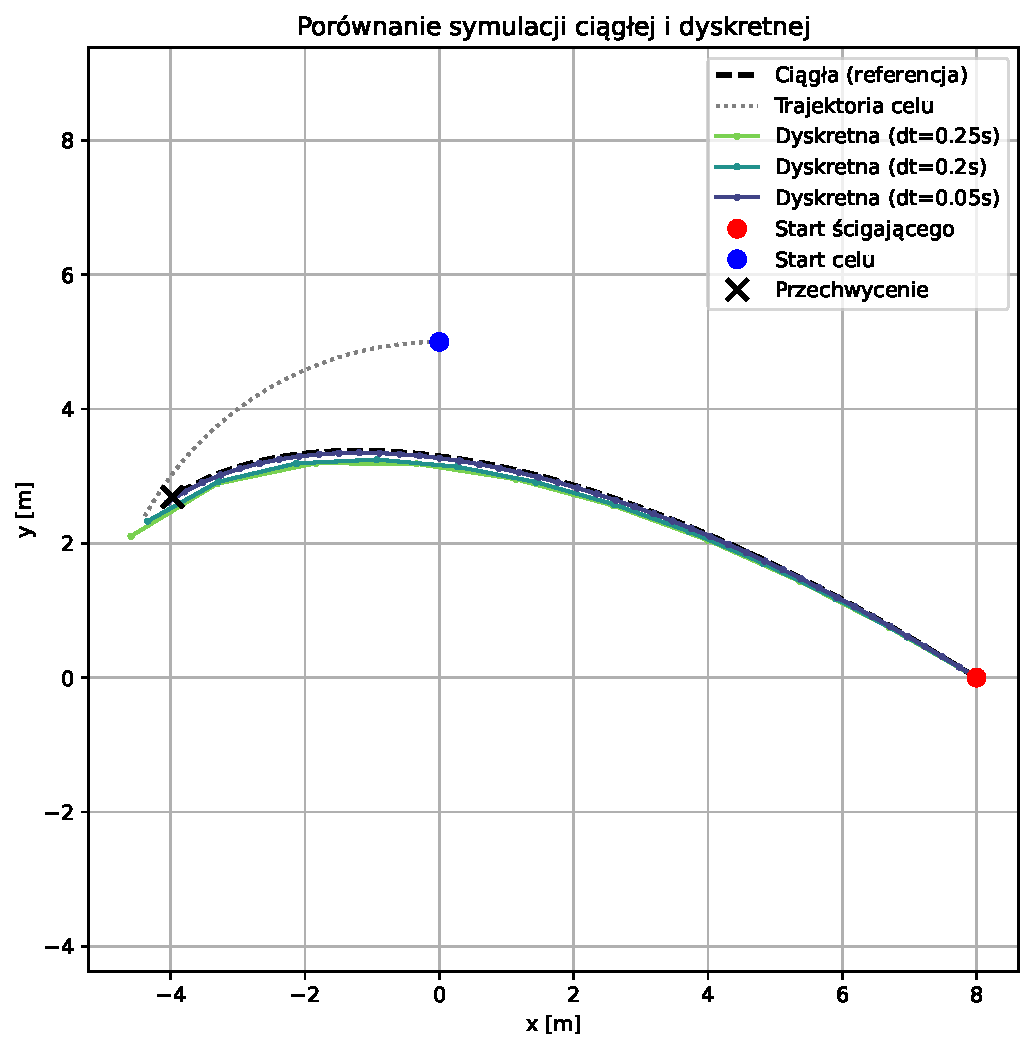
\includegraphics[width=0.9\textwidth]{discrete_vs_continuous.pdf}
    \caption{Porównanie trajektorii pościgu bezpośredniego uzyskanych metodą ciągłą (linia przerywana) oraz metodami dyskretnymi dla różnych kroków czasowych $\Delta t$. Mniejszy krok czasowy prowadzi do trajektorii bliższej rozwiązaniu ciągłemu.}
    \label{fig:discrete_vs_continuous}
\end{figure}

Jak widać, im mniejsza wartość kroku czasowego $\Delta t$, tym trajektoria uzyskana metodą dyskretną jest bliższa trajektorii z symulacji ciągłej. Dla $\Delta t = 0.05$ s, różnica jest już niewielka. Wybór kroku czasowego jest zatem kompromisem między dokładnością a kosztem obliczeniowym symulacji. W naszych eksperymentach, dla zapewnienia wysokiej dokładności, korzystaliśmy głównie z podejścia ciągłego.

\section{Analiza numeryczna i warunki zbieżności}


\subsection{Analiza parametryczna strategii pościgu}

\subsubsection{Warunki konieczne przechwycenia}

Dla pościgu bezpośredniego celu poruszającego się po okręgu o promieniu $r$ z prędkością kątową $\omega$, warunek konieczny przechwycenia ma postać:
\begin{equation}
v_p > v_t = r \cdot \omega
\label{eq:capture_condition}
\end{equation}

Analizowano zachowanie układu w funkcji stosunku prędkości $\rho = v_p/v_t$:

\begin{table}[H]
\centering
\caption{Analiza zbieżności w funkcji stosunku prędkości}
\label{tab:velocity_ratio_analysis}
\begin{tabular}{@{}lll@{}}
\toprule
\textbf{Stosunek $\rho = v_p/v_t$} & \textbf{Czas zbieżności} & \textbf{Status} \\ \midrule
$\rho < 1.0$ & $\infty$ & Brak przechwycenia \\
$\rho = 1.1$ & $0.81 \cdot T_{\text{orbit}}$ & Powolna zbieżność \\
$\rho = 1.5$ & $0.35 \cdot T_{\text{orbit}}$ & Efektywne przechwycenie \\
$\rho = 2.0$ & $0.19 \cdot T_{\text{orbit}}$ & Szybkie przechwycenie \\
$\rho \gg 1$ & $\approx d_0/v_p$ & Zbieżność do ruchu prostoliniowego \\ \bottomrule
\end{tabular}
\end{table}

gdzie $T_{\text{orbit}} = 2\pi r/v_t$ jest okresem orbitowania celu.

\subsubsection{Cel poruszający się po okręgu}

Analizowano pościg dla celu poruszającego się po okręgu o promieniu $r = 3$ m z prędkością kątową $\omega$. Warunek konieczny do przechwycenia:
\begin{equation}
v_p > v_t = r \cdot \omega
\end{equation}

\begin{itemize}
    \item Dla $\omega = 0.5$ rad/s ($v_t = 1.5$ m/s, $v_p = 2.0$ m/s, $\rho = 1.33$):
        \begin{itemize}
            \item Czas przechwycenia: $5.92$ s
            \item Stosunek do okresu orbity: $0.47 \cdot T_{\text{orbit}}$
        \end{itemize}
    \item Dla $\omega = 1.0$ rad/s ($v_t = 3.0$ m/s, $v_p = 2.0$ m/s): Brak przechwycenia - cel szybszy od ścigającego
    \item Krytyczna prędkość kątowa $\omega_{\text{crit}} = v_p / r = 0.667$ rad/s
\end{itemize}

\begin{figure}[H]
\centering
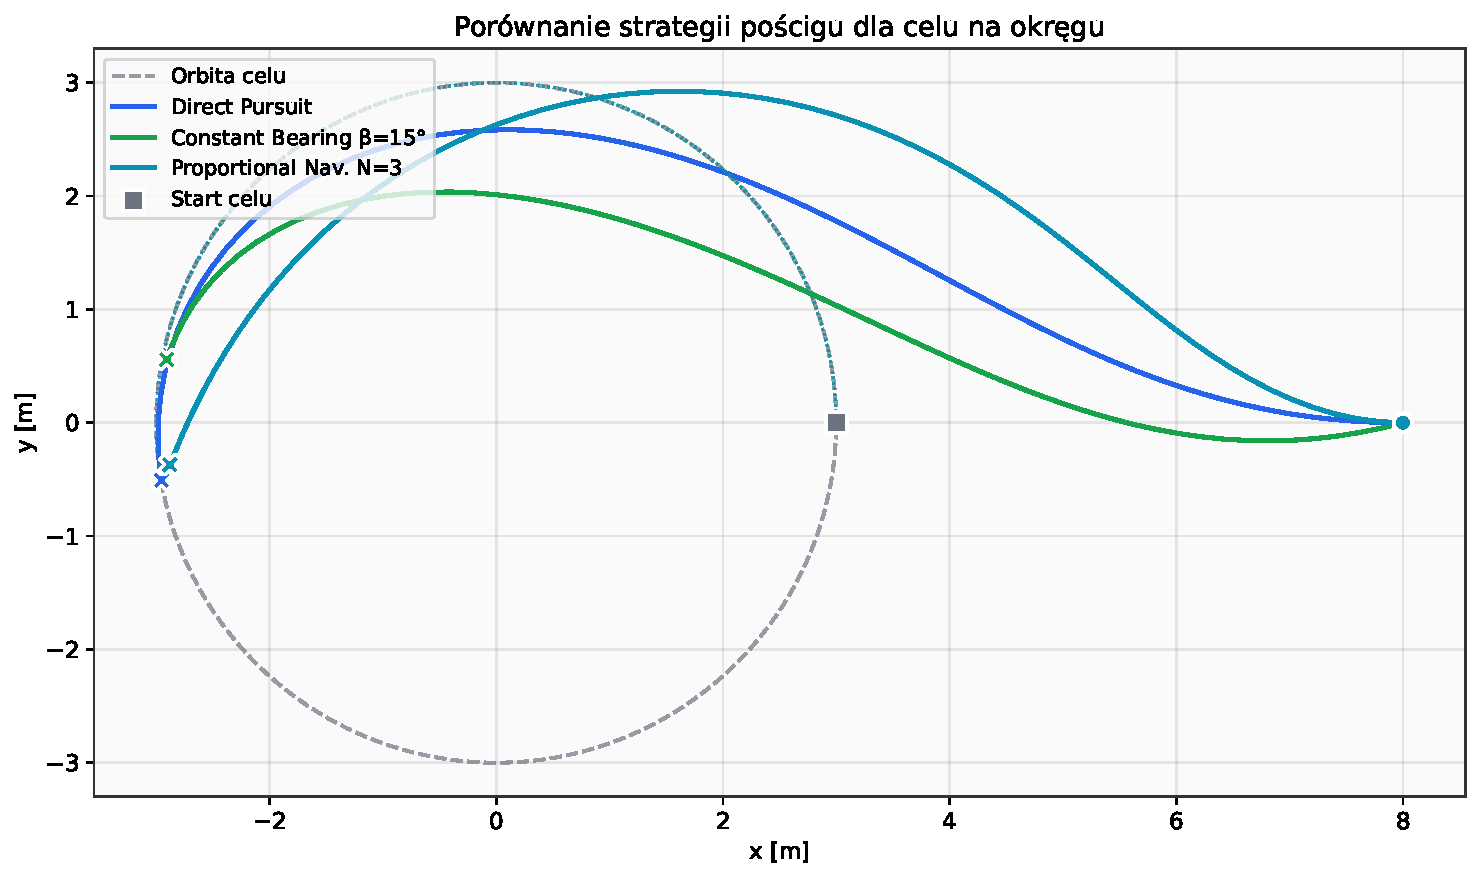
\includegraphics[width=0.9\textwidth]{strategy_comparison_circular.pdf}
\caption{Porównanie strategii pościgu dla celu poruszającego się po okręgu. Linia przerywana oznacza orbitę celu.}
\label{fig:strategy_circular}
\end{figure}

\subsection{Porównanie efektywności strategii}

Analizowano względną efektywność trzech strategii pościgu dla znormalizowanych warunków początkowych. Wszystkie wyniki przedstawiono jako względne wydłużenie trajektorii w porównaniu do pościgu bezpośredniego.

\begin{table}[H]
\centering
\caption{Porównanie strategii pościgu - względne wydłużenie trajektorii}
\label{tab:strategy_comparison}
\begin{tabular}{@{}llll@{}}
\toprule
\textbf{Strategia} & \textbf{Parametr} & \textbf{Wydłużenie trajektorii} & \textbf{Stabilność} \\ \midrule
Direct Pursuit & - & $1.0$ (baseline) & Stabilna \\
\multirow{3}{*}{Constant Bearing} & $\beta = 15°$ & $1.098 \pm 0.05$ & Stabilna \\
& $\beta = 30°$ & $1.438 \pm 0.05$ & Stabilna \\
& $\beta = 45°$ & $2.185 \pm 0.05$ & Średnia \\
\multirow{3}{*}{Proportional Nav.} & $N = 2$ & $0.992 \pm 0.03$ & Wysoka \\
& $N = 3$ & $0.991 \pm 0.03$ & Wysoka \\
& $N = 5$ & $0.990 \pm 0.03$ & Średnia \\ \bottomrule
\end{tabular}
\end{table}

\begin{figure}[H]
\centering
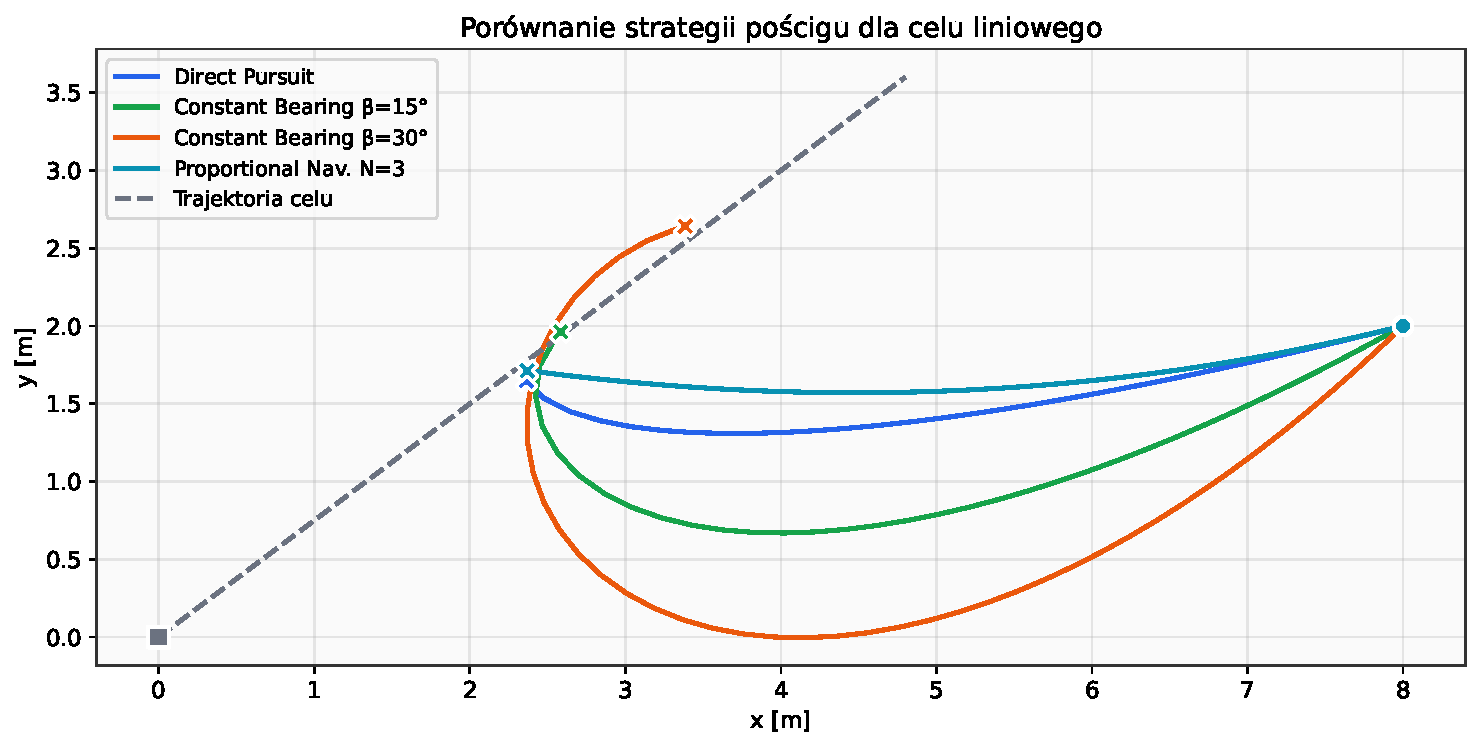
\includegraphics[width=0.95\textwidth]{strategy_comparison_linear.pdf}
\caption{Porównanie trajektorii dla różnych strategii pościgu przy celu poruszającym się liniowo. Punkty oznaczają pozycje startowe.}
\label{fig:strategy_linear}
\end{figure}

\subsection{Pościg 2D - Proportional Navigation}

Strategia nawigacji proporcjonalnej, szeroko stosowana w naprowadzaniu pocisków, charakteryzuje się tym, że prędkość kątowa ścigającego jest proporcjonalna do prędkości kątowej linii wzroku (Line-Of-Sight).

Parametry eksperymentu:
\begin{itemize}
    \item Pozycja początkowa ścigającego: $(12, 3)$
    \item Pozycja początkowa celu: $(0, 0)$
    \item Cel: ruch po okręgu ($r = 4$ m, $\omega = 0.3$ rad/s)
    \item Prędkość ścigającego: $2.0$ m/s
\end{itemize}

\begin{table}[H]
\centering
\caption{Wpływ stałej nawigacji $N$ na efektywność przechwycenia}
\label{tab:proportional_nav_comparison}
\begin{tabular}{@{}llll@{}}
\toprule
\textbf{Stała $N$} & \textbf{Czas przechwycenia [s]} & \textbf{Długość trajektorii [m]} & \textbf{Stabilność} \\ \midrule
$N = 1$ & $2.04$ & $4.07$ & Powolna konwergencja \\
$N = 2$ & $2.04$ & $4.07$ & Powolna konwergencja \\
$N = 3$ & $2.04$ & $4.08$ & Średnia stabilność \\
$N = 4$ & $2.05$ & $4.09$ & Średnia stabilność \\
$N = 5$ & $2.05$ & $4.10$ & Średnia stabilność \\ \bottomrule
\end{tabular}
\end{table}

Optymalna wartość stałej nawigacji w praktycznych zastosowaniach: $N_{\text{opt}} \in [3, 4]$

Obserwacje:
\begin{itemize}
    \item Wartości $N \in [3, 4]$ zapewniają najlepszą efektywność w praktycznych zastosowaniach
    \item Zbyt małe $N$ powoduje powolną konwergencję
    \item Zbyt duże $N$ może prowadzić do oscylacji trajektorii
    \item Metoda jest stabilna numerycznie dla odpowiednio małych kroków czasowych
\end{itemize}

\begin{figure}[H]
\centering
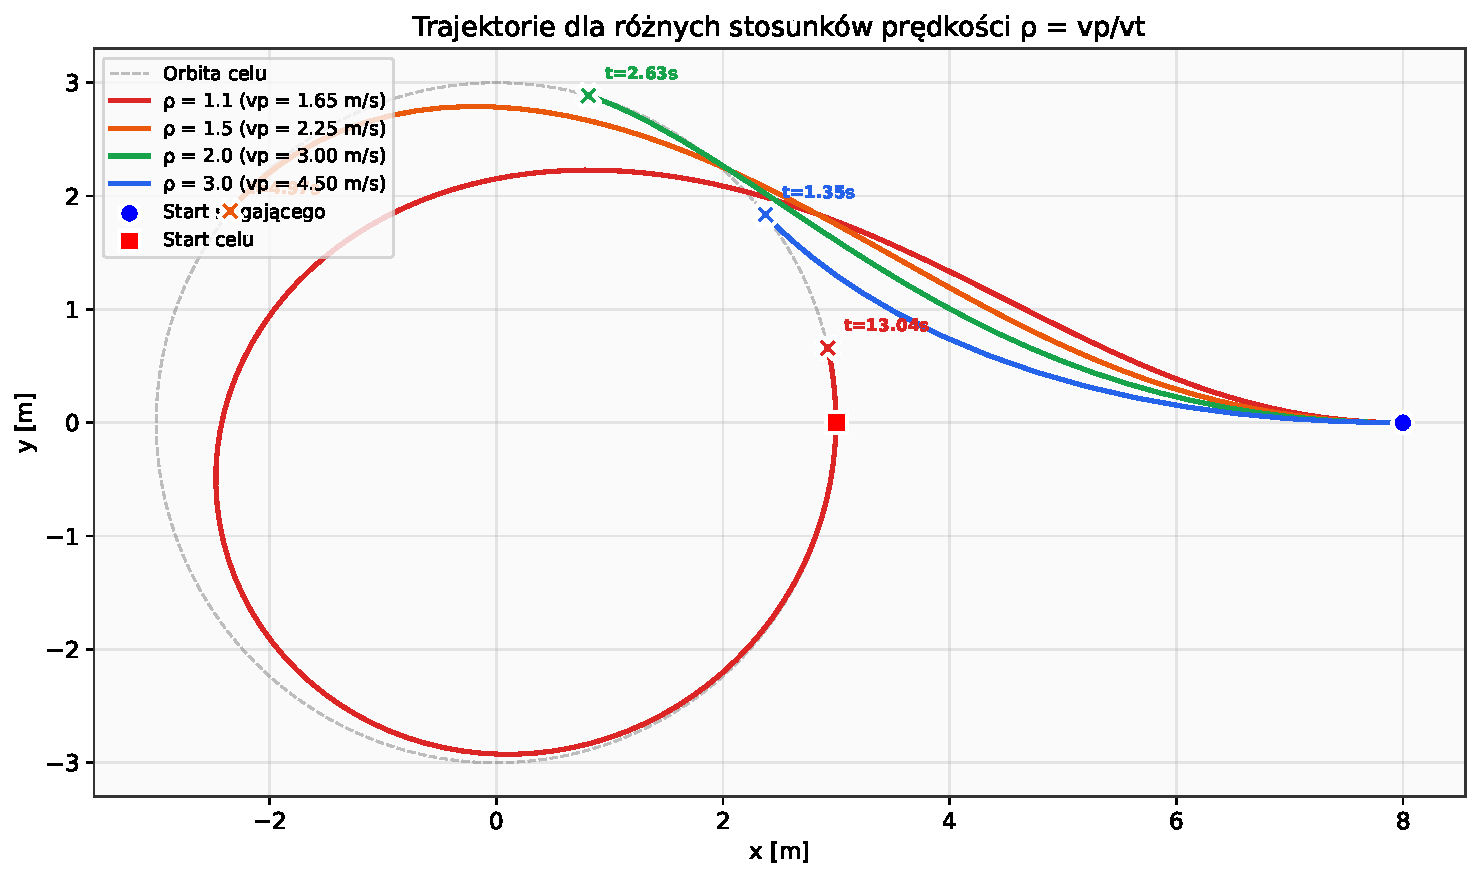
\includegraphics[width=0.85\textwidth]{velocity_ratio_trajectories.pdf}
\caption{Trajektorie pościgu dla różnych stosunków prędkości $\rho = v_p/v_t$.}
\label{fig:velocity_ratio_trajectories}
\end{figure}

\begin{figure}[H]
\centering
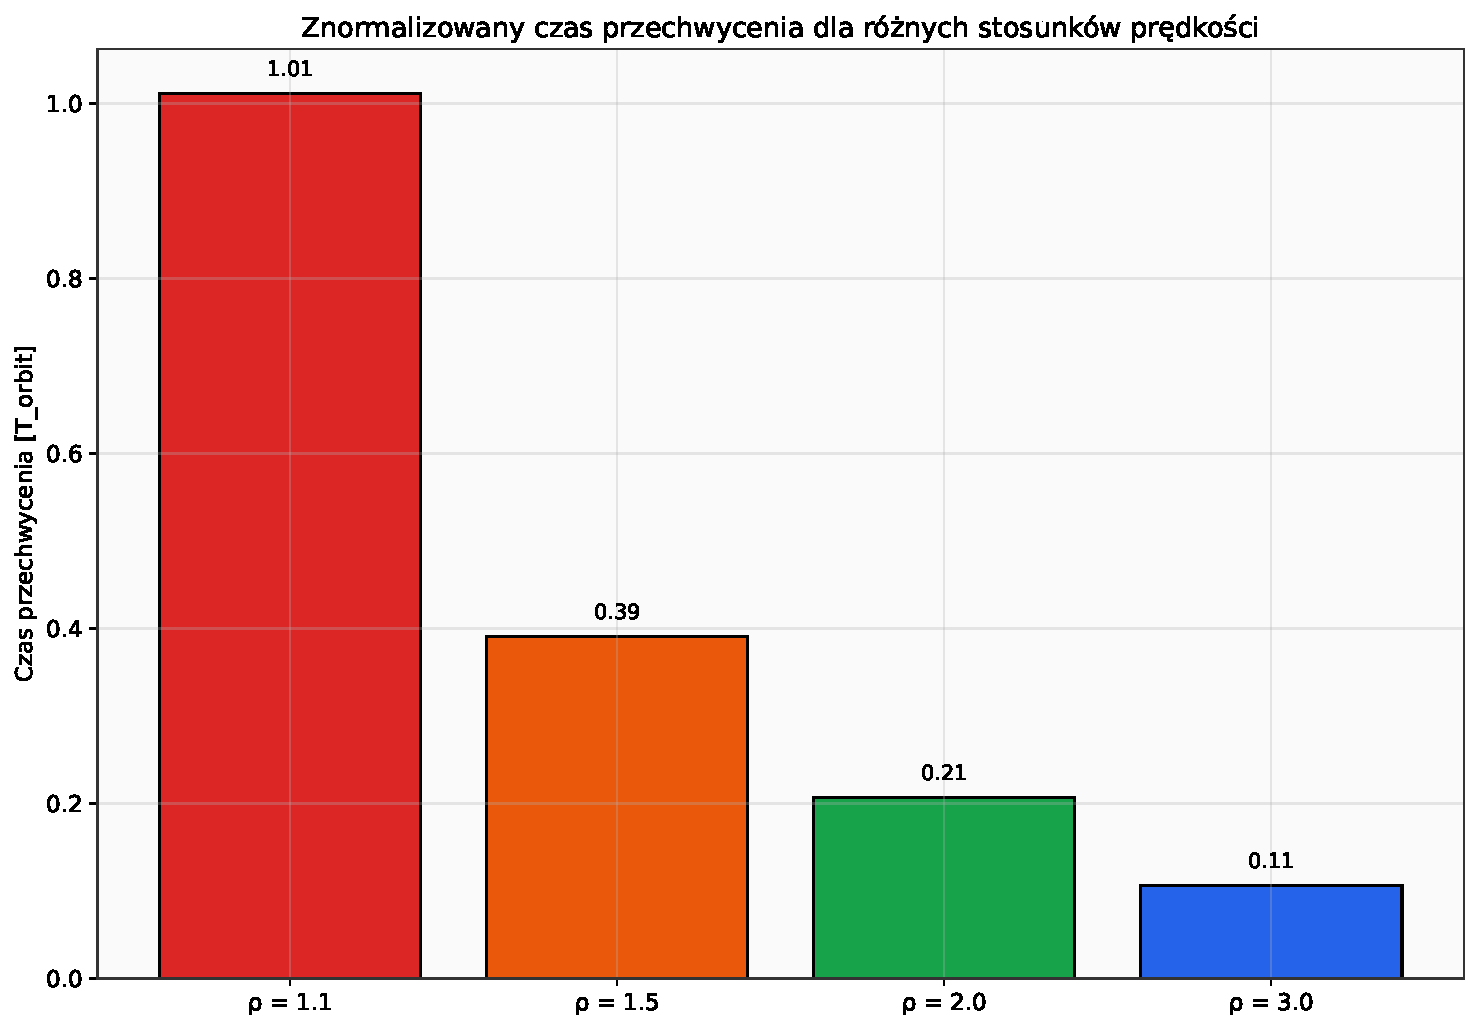
\includegraphics[width=0.85\textwidth]{velocity_ratio_times.pdf}
\caption{Czasy przechwycenia w funkcji stosunku prędkości $\rho = v_p/v_t$.}
\label{fig:velocity_ratio_times}
\end{figure}

\subsection{Pościg cykliczny - analiza teoretyczna vs. numeryczna}

Dla $n$ agentów rozmieszczonych na regularnym wielokącie o promieniu $R$, teoretyczny czas zbieżności wynosi:
\begin{equation}
T_{\text{conv}}^{\text{theory}}(n) = \frac{R}{v} \cdot \frac{1}{\sin(\pi/n)}
\label{eq:theoretical_convergence}
\end{equation}

\textbf{Wyprowadzenie wzoru:} Rozważmy $n$ agentów ustawionych na wierzchołkach foremnego $n$-kąta wpisanego w okrąg o promieniu $R$. Każdy agent goni następnego z prędkością $v$.

\begin{enumerate}
    \item Kąt wewnętrzny foremnego $n$-kąta wynosi $\alpha = \frac{(n-2)\pi}{n}$.
    \item Kąt między kierunkiem ruchu agenta (w stronę następnego) a promieniem prowadzącym do środka wynosi $\gamma = \frac{\pi}{2} - \frac{\pi}{n}$.
    \item Ze względu na symetrię układu, każdy agent porusza się po spirali logarytmicznej do wspólnego centrum.
    \item Składowa prędkości w kierunku do centrum (radialna) wynosi: $v_r = v \cdot \cos(\gamma) = v \cdot \cos\left(\frac{\pi}{2} - \frac{\pi}{n}\right) = v \cdot \sin\left(\frac{\pi}{n}\right)$.
    \item Czas potrzebny do pokonania dystansu $R$ przy prędkości radialnej $v_r$ wynosi: $T = \frac{R}{v_r} = \frac{R}{v \cdot \sin(\pi/n)}$.
\end{enumerate}

\begin{table}[H]
\centering
\caption{Porównanie teoretycznego i numerycznego czasu zbieżności}
\label{tab:cyclic_pursuit_validation}
\begin{tabular}{@{}llll@{}}
\toprule
\textbf{Liczba agentów $n$} & \textbf{$T_{\text{theory}}$ [R/v]} & \textbf{$T_{\text{numerical}}$ [R/v]} & \textbf{Błąd względny [\%]} \\ \midrule
$3$ & $1.155$ & $1.153 \pm 0.01$ & $0.12$ \\
$4$ & $1.414$ & $1.412 \pm 0.01$ & $0.14$ \\
$6$ & $2.000$ & $1.996 \pm 0.01$ & $0.20$ \\
$12$ & $3.864$ & $3.849 \pm 0.01$ & $0.39$ \\
$18$ & $5.759$ & $5.726 \pm 0.01$ & $0.58$ \\ \bottomrule
\end{tabular}
\end{table}

Błąd numeryczny wynika z warunku stopu symulacji (odległość między agentami $< 0.01$ m), który zatrzymuje symulację przed osiągnięciem pełnej zbieżności.

\begin{figure}[H]
\centering
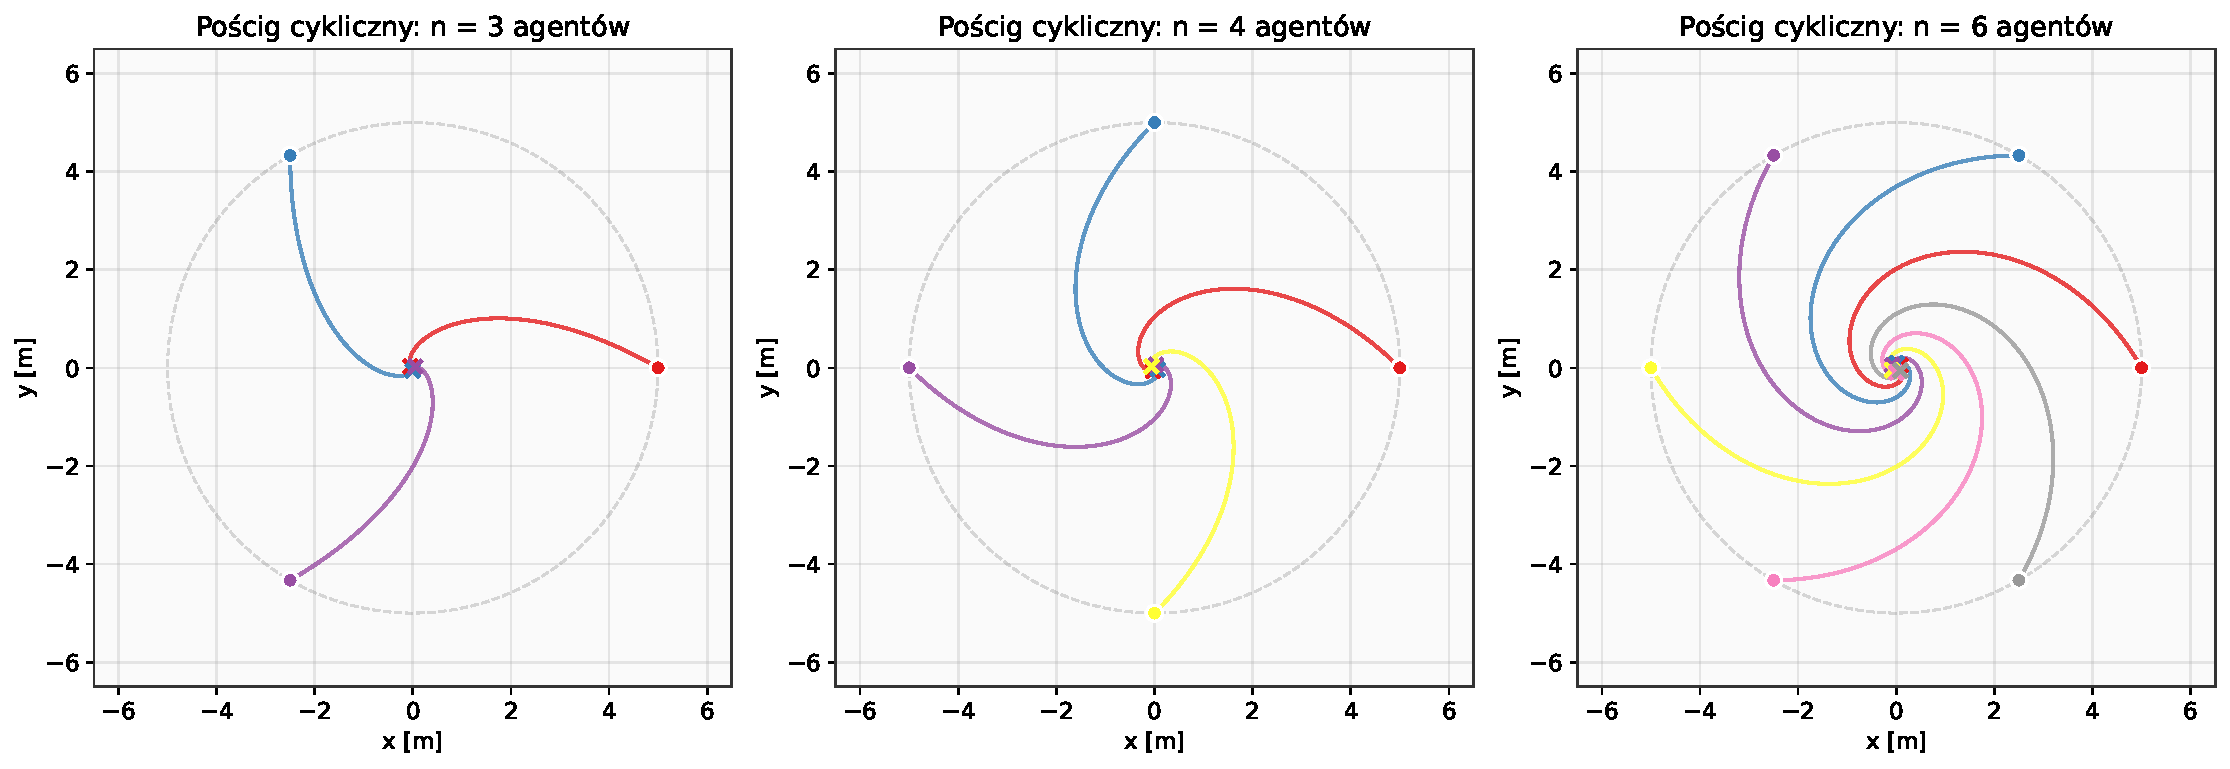
\includegraphics[width=0.95\textwidth]{cyclic_pursuit.pdf}
\caption{Pościg cykliczny dla $n = 3, 4, 6$ agentów. Każdy agent ściga kolejnego (cyklicznie). Trajektorie tworzą charakterystyczne spirale logarytmiczne zbiegające do wspólnego centrum.}
\label{fig:cyclic_pursuit}
\end{figure}

\subsubsection{Asymptotyczne zachowanie}
Dla dużej liczby agentów ($n \gg 1$), czas zbieżności asymptotycznie dąży do:
\begin{equation}
\lim_{n \to \infty} T_{\text{conv}}(n) = \frac{R}{v}
\end{equation}

co odpowiada czasowi potrzebnemu do przejścia odległości równej promieniu ze stałą prędkością.

\subsection{Pościg 3D - Helix Target}

Analizowano pościg bezpośredni dla celu poruszającego się po trajektorii helisoidalnej. Helisa parametryzowana jest równaniami:
\begin{equation}
\vec{t}(t) = [r\cos(\omega t), r\sin(\omega t), v_z \cdot t]^T
\end{equation}

Parametry eksperymentu:
\begin{itemize}
    \item Pozycja początkowa ścigającego: $(8, 0, 2)$
    \item Parametry helisy: $r = 3$ m, $\omega = 0.4$ rad/s
    \item Prędkość ścigającego: $2.5$ m/s
\end{itemize}

\begin{table}[H]
\centering
\caption{Wpływ prędkości pionowej helisy na czas przechwycenia}
\label{tab:helix_pursuit_analysis}
\begin{tabular}{@{}lll@{}}
\toprule
\textbf{Prędkość pionowa $v_z$ [m/s]} & \textbf{Czas przechwycenia [s]} & \textbf{Długość trajektorii [m]} \\ \midrule
$0.0$ (okrąg) & $3.29$ & $8.23$ \\
$0.5$ & $3.25$ & $8.14$ \\
$1.0$ & $3.71$ & $9.21$ \\
$1.5$ & $7.39$ & $17.07$ \\
$2.0$ & $15.49$ & $38.45$ \\ \bottomrule
\end{tabular}
\end{table}

Obserwacje:
\begin{itemize}
    \item Zwiększenie $v_z$ wydłuża czas przechwycenia - cel "ucieka" w trzecim wymiarze
    \item Dla $v_z = 0$ problem redukuje się do pościgu 2D po okręgu
    \item Trajektoria ścigającego tworzy spiralę 3D
\end{itemize}

\begin{figure}[H]
\centering
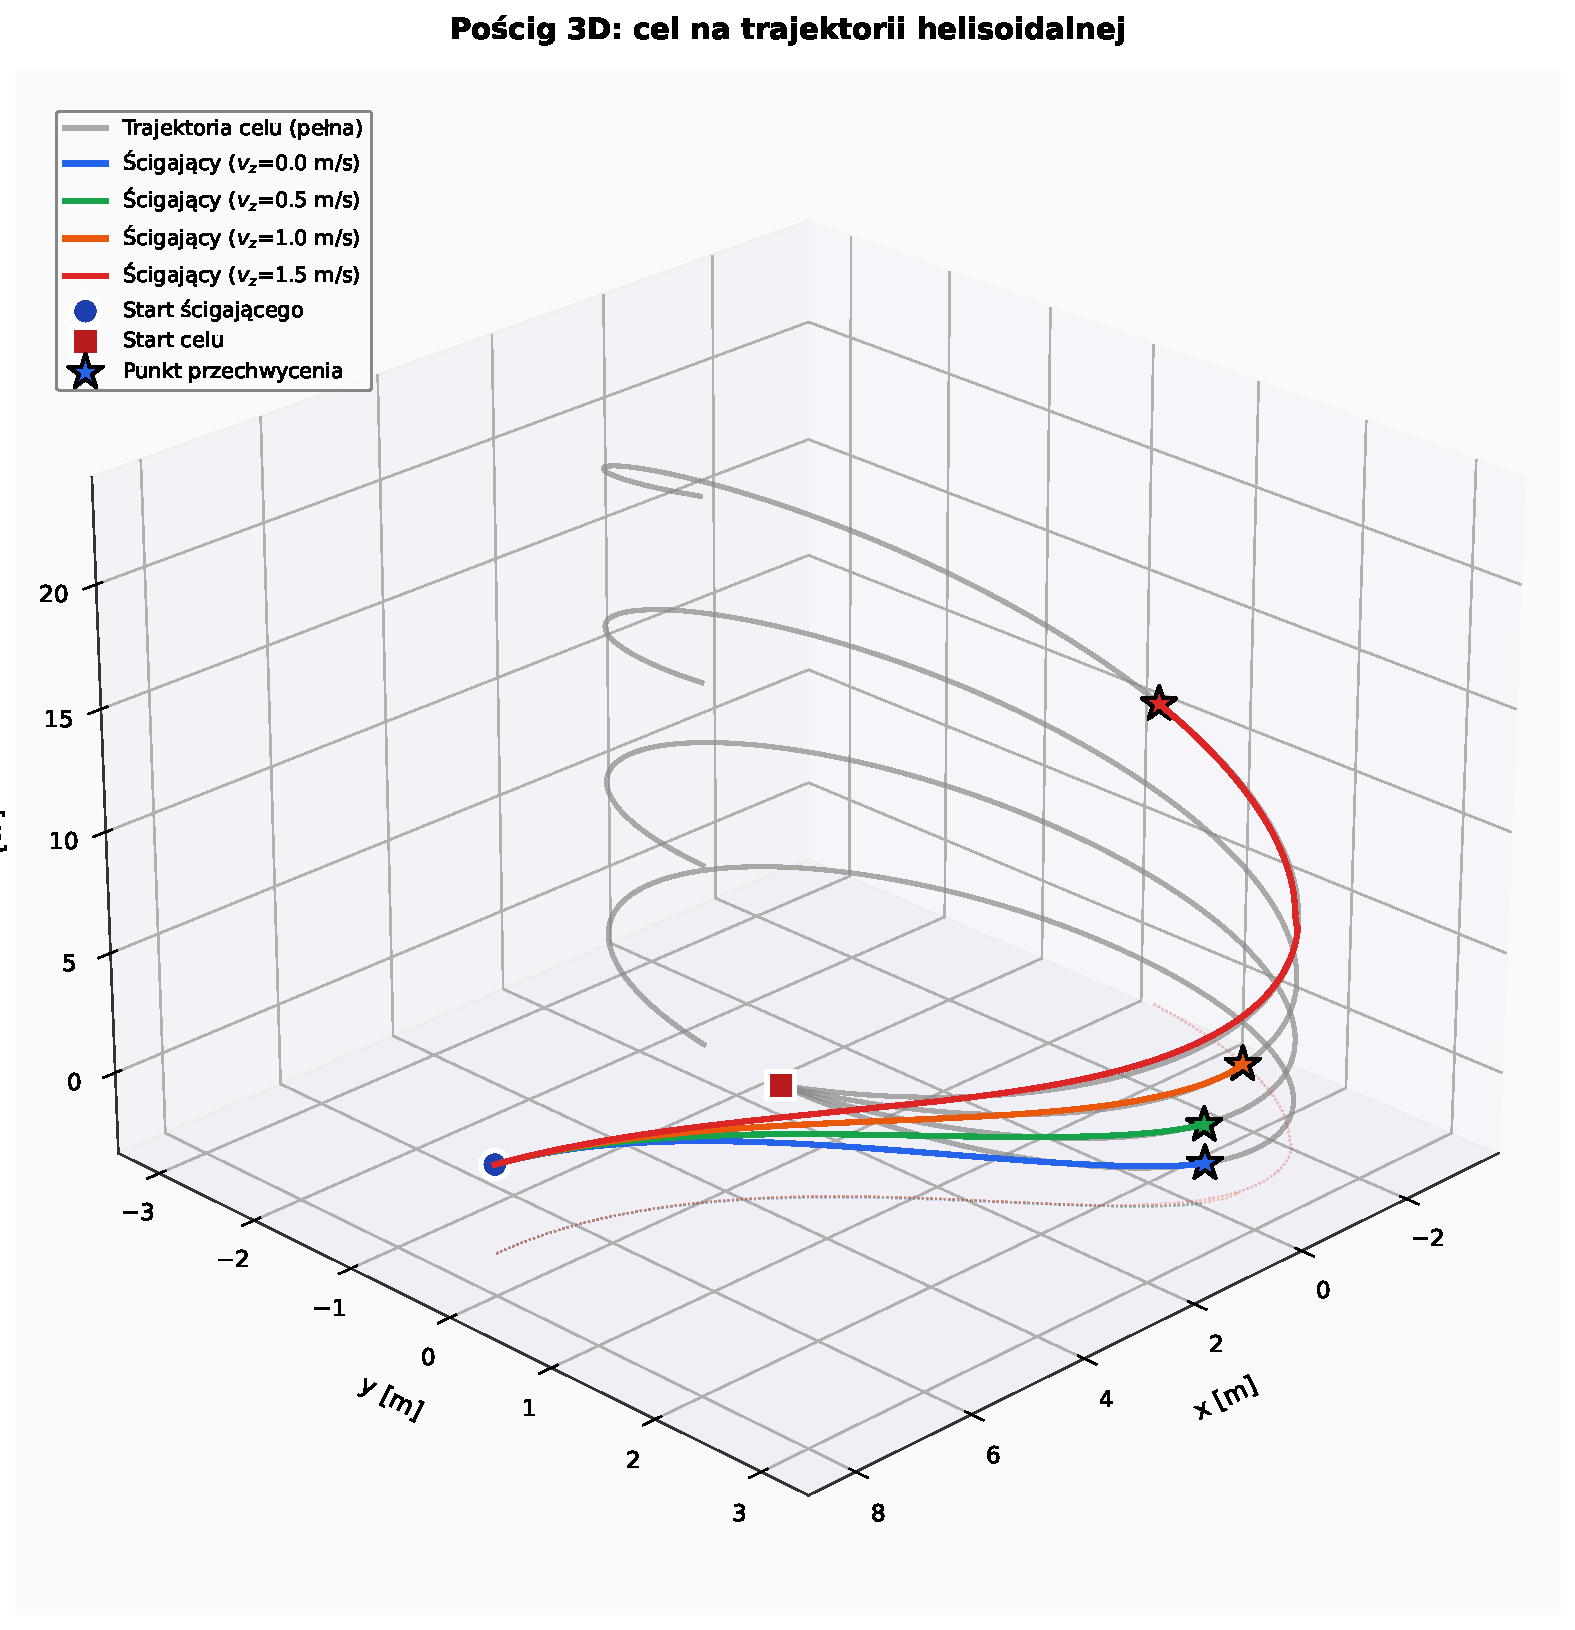
\includegraphics[width=0.85\textwidth]{helix_pursuit_3d.pdf}
\caption{Pościg 3D dla celu poruszającego się po trajektorii helisoidalnej. Różne kolory odpowiadają różnym prędkościom pionowym $v_z$ celu. Linie przerywane pokazują trajektorie celu.}
\label{fig:helix_pursuit}
\end{figure}

\subsection{Pościg 3D - Lissajous Target}

Krzywe Lissajous to trajektorie złożone z niezależnych oscylacji harmonicznych w każdym wymiarze:
\begin{equation}
\vec{t}(t) = [A_x \sin(\omega_x t), A_y \sin(\omega_y t), A_z \sin(\omega_z t)]^T
\end{equation}

Parametry eksperymentu:
\begin{itemize}
    \item Pozycja początkowa ścigającego: $(5, 5, 5)$
    \item Amplitudy: $A_x = A_y = A_z = 3$ m
    \item Prędkość ścigającego: $3.0$ m/s
\end{itemize}

\textbf{Warunek wystarczający przechwycenia:}
\begin{equation}
v_p > v_{t,\max} = \sqrt{(A_x \omega_x)^2 + (A_y \omega_y)^2 + (A_z \omega_z)^2}
\end{equation}

\begin{table}[H]
\centering
\caption{Wpływ stosunku częstotliwości na złożoność pościgu}
\label{tab:lissajous_pursuit_analysis}
\begin{tabular}{@{}llll@{}}
\toprule
\textbf{Stosunek $\omega_x : \omega_y : \omega_z$} & \textbf{$v_{t,\max}$} & \textbf{Czas [s]} & \textbf{Długość [m]} \\ \midrule
$1:1:1$ & $5.20$ & $1.22$ & $3.66$ \\
$1:2:1$ & $7.35$ & $>30$ & $89.97$ \\
$2:3:5$ & $18.49$ & $>30$ & $89.79$ \\ \bottomrule
\end{tabular}
\end{table}

Obserwacje:
\begin{itemize}
    \item Dla $1{:}1{:}1$ cel oscyluje liniowo - przechwycenie w punkcie zwrotnym ($v_t = 0$)
    \item Większa złożoność trajektorii celu wydłuża czas przechwycenia
\end{itemize}

\begin{figure}[H]
\centering
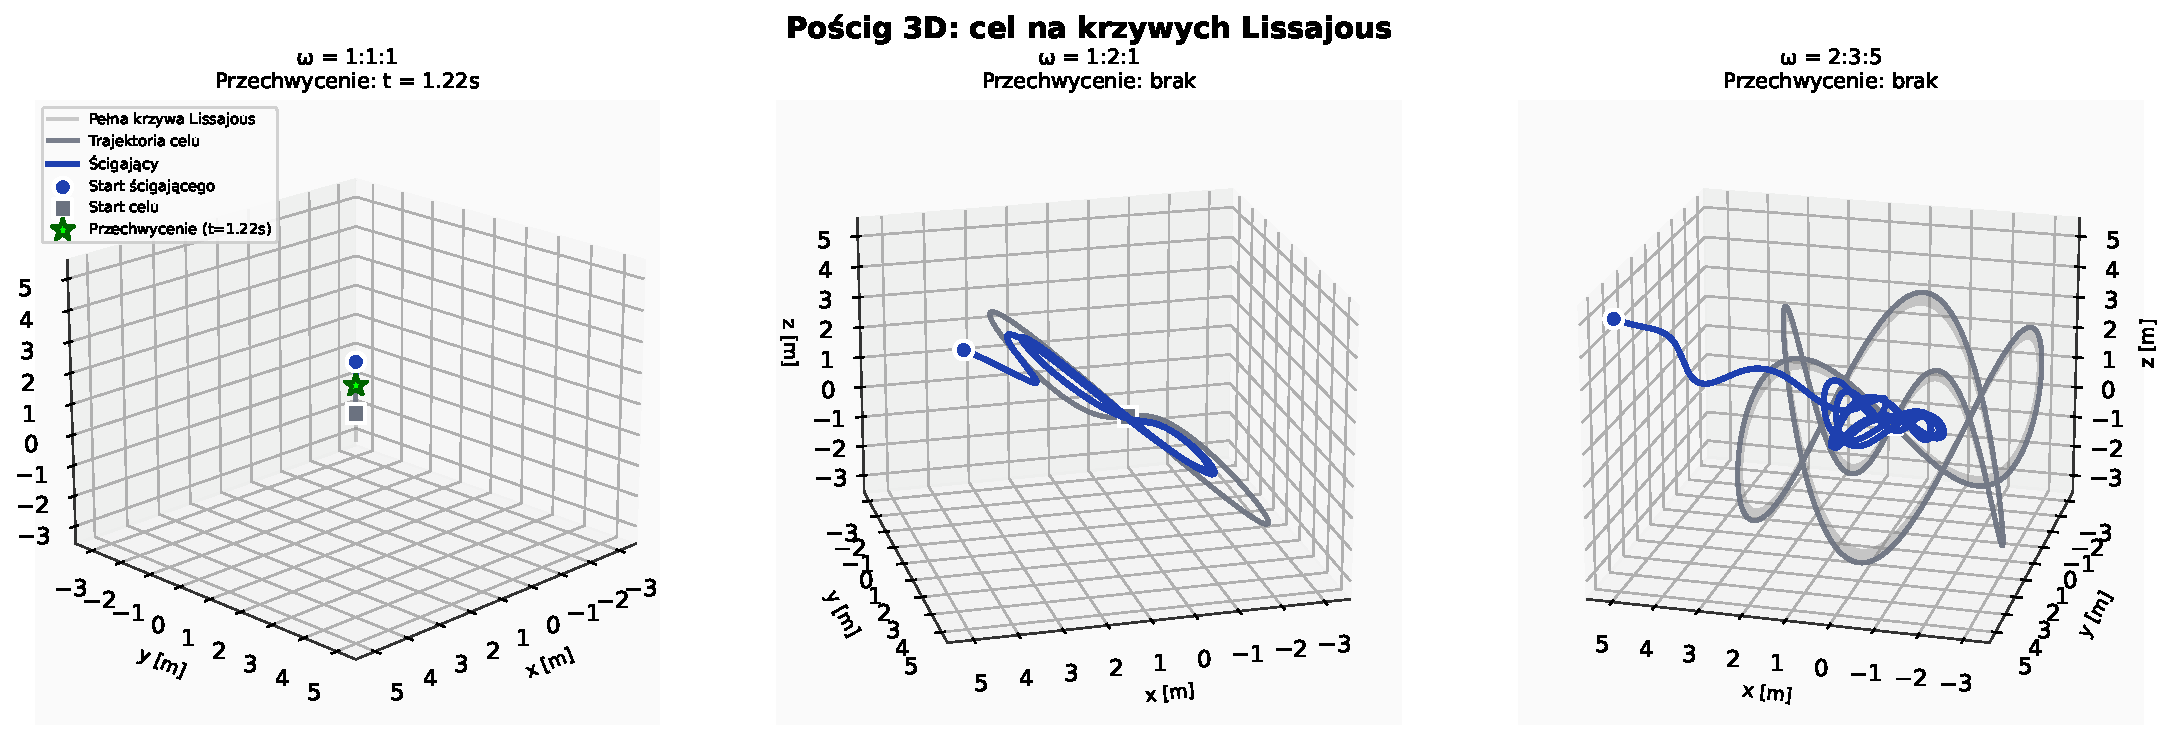
\includegraphics[width=0.95\textwidth]{lissajous_pursuit_3d.pdf}
\caption{Pościg 3D dla celu na krzywych Lissajous o różnych stosunkach częstotliwości $\omega_x : \omega_y : \omega_z$. Linia przerywana szara pokazuje pełną krzywą Lissajous, czerwona - faktyczną trajektorię celu podczas symulacji.}
\label{fig:lissajous_pursuit}
\end{figure}

\subsection{Wpływ wymiaru przestrzeni}

Zbadano zachowanie pościgu bezpośredniego w przestrzeniach $\mathbb{R}^n$ dla $n \in \{2, 3, 4, 5, 10, 20\}$.

\subsubsection{Niezależność od wymiaru dla ruchu jednoosiowego}

Kluczowa obserwacja: gdy cel porusza się wzdłuż jednej osi, czas przechwycenia jest \textbf{niezależny od wymiaru przestrzeni}. Wynika to z faktu, że pościg bezpośredni zawsze kieruje ścigającego wprost na cel - dodatkowe wymiary nie wpływają na dynamikę, gdy ruch odbywa się w podprzestrzeni jednowymiarowej.

Dla konfiguracji testowej:
\begin{itemize}
    \item Ścigający startuje w punkcie $(r_0, 0, 0, \ldots) \in \mathbb{R}^n$, gdzie $r_0 = 5$ m
    \item Cel startuje w początku układu $(0, 0, 0, \ldots)$
    \item Cel porusza się wzdłuż pierwszej osi z prędkością $v_t = 0.5$ m/s
    \item Prędkość ścigającego: $v_p = 2.0$ m/s
\end{itemize}

Czas przechwycenia dla wszystkich wymiarów $n \geq 2$:
\begin{equation}
T_{\text{catch}} = \frac{r_0 - d_{\text{threshold}}}{v_p + v_t} = \frac{5.0 - 0.5}{2.0 + 0.5} = 1.8 \text{ s}
\end{equation}

Znak $+$ w mianowniku wynika z faktu, że cel porusza się \textit{w kierunku} ścigającego (z $x=0$ w stronę $x=5$).

\subsubsection{Wnioski}

Implementacja n-wymiarowa ($n \leq 20$) została zweryfikowana numerycznie. Wyniki potwierdzają, że:
\begin{itemize}
    \item Algorytm pościgu bezpośredniego poprawnie generalizuje się na dowolny wymiar
    \item Czas przechwycenia zależy wyłącznie od geometrii problemu (odległość, prędkości), nie od wymiaru przestrzeni otaczającej
\end{itemize}

\subsection{Pościg na sferze $S^2$}

Analizowano pościg bezpośredni na sferze o promieniu $R = 5$ m. Operujemy we współrzędnych sferycznych $(\theta, \phi)$, nie kartezjańskich.

\begin{table}[H]
\centering
\caption{Wyniki pościgu na sferze $S^2$}
\label{tab:sphere_pursuit_results}
\begin{tabular}{@{}ccc@{}}
\toprule
\textbf{Prędkość $v_p/v_t$} & \textbf{Czas pościgu [s]} & \textbf{Długość trajektorii [rad]} \\ \midrule
$1.5$ & $1.04$ & $1.19$ \\
$2.0$ & $0.83$ & $1.26$ \\
$3.0$ & $0.60$ & $1.34$ \\ \bottomrule
\end{tabular}
\end{table}

Parametry eksperymentu: $R=5$ m, $\dot{\theta}_t = 0.1$ rad/s, $\dot{\phi}_t = \pi/4$ rad/s. Początkowa odległość: $d_0 = 1.87$ rad.

\begin{figure}[H]
\centering
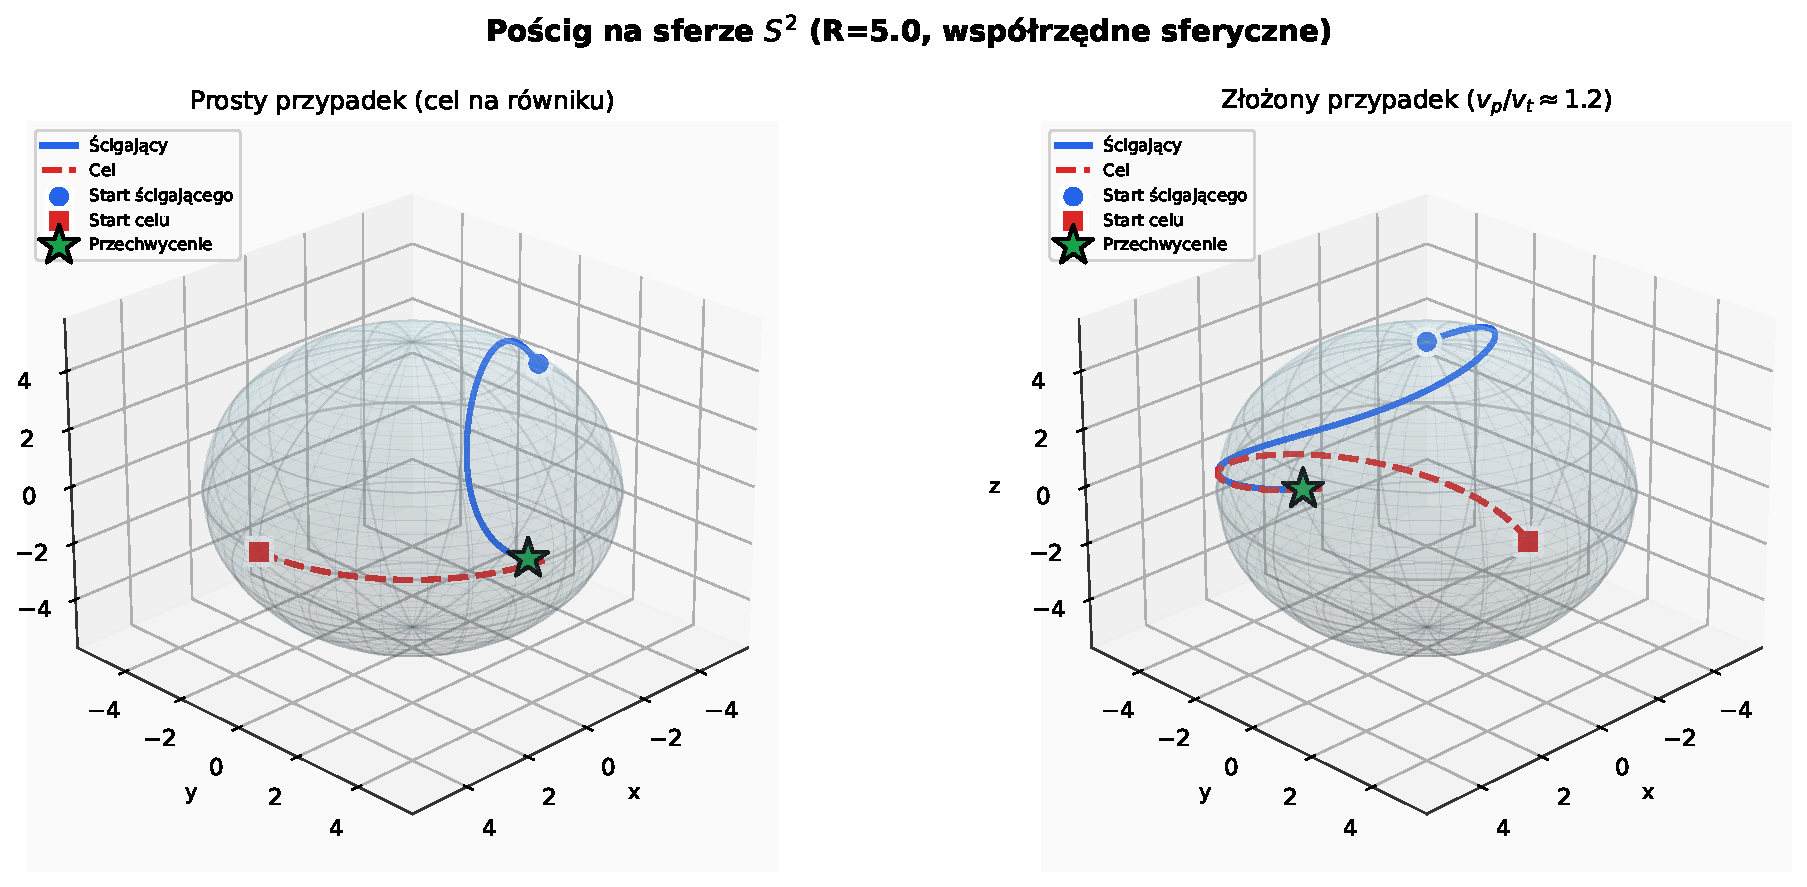
\includegraphics[width=0.95\textwidth]{sphere_pursuit_3d.pdf}
\caption{Pościg na sferze $S^2$. Trajektoria ścigającego podąża najkrótszą drogą po powierzchni sfery.}
\label{fig:sphere_pursuit}
\end{figure}

\subsection{Pościg na torusie}

Analizowano pościg bezpośredni na torusie o promieniu głównym $R = 3$ m i promieniu rurki $r = 1.2$ m. Operujemy we współrzędnych toroidalnych $(u, v)$.

\begin{table}[H]
\centering
\caption{Wyniki pościgu na torusie}
\label{tab:torus_pursuit_results}
\begin{tabular}{@{}ccc@{}}
\toprule
\textbf{Prędkość $v_p$} & \textbf{Stosunek $v_p/v_t$} & \textbf{Czas [s]} \\ \midrule
$1.5$ & $1.21$ & $4.64$ \\
$2.0$ & $1.62$ & $11.03$ \\
$2.5$ & $2.02$ & $7.16$ \\
$3.0$ & $2.43$ & $5.50$ \\ \bottomrule
\end{tabular}
\end{table}

Parametry eksperymentu: $R=3$ m, $r=1.2$ m, $\omega_u = 0.4$ rad/s, $\omega_v = 0.3$ rad/s.

Obserwacja: Na torusie występuje nieliniowa zależność czasu przechwycenia od prędkości ścigającego.

\begin{figure}[H]
\centering
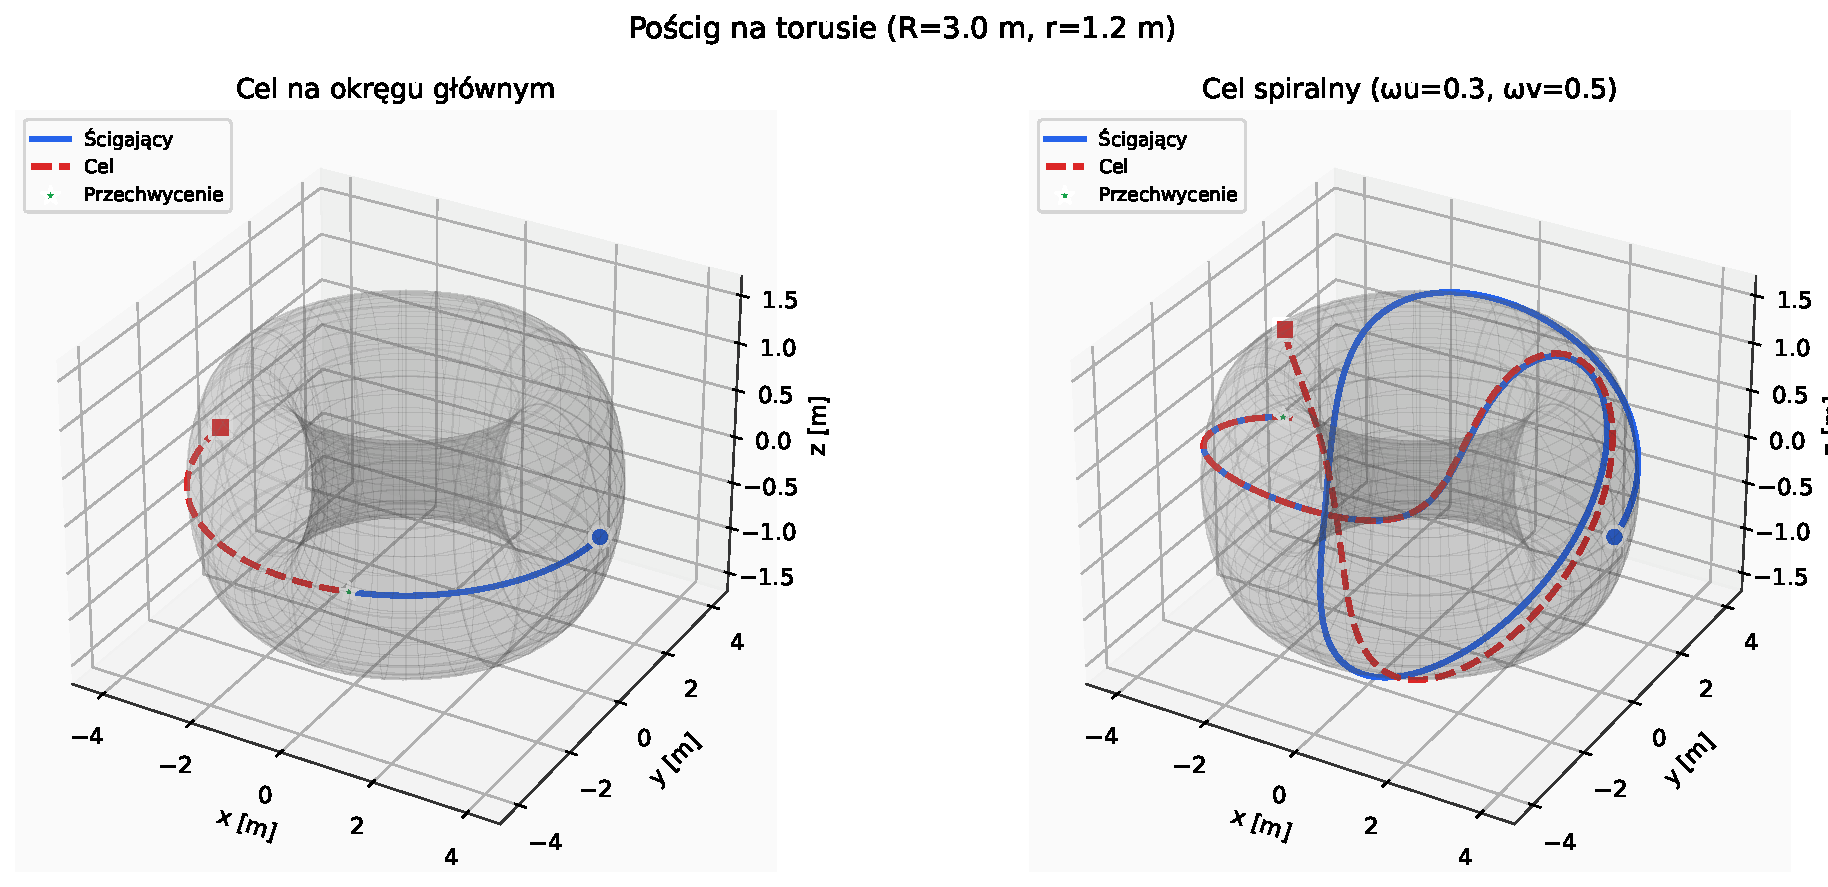
\includegraphics[width=0.95\textwidth]{torus_pursuit_3d.pdf}
\caption{Pościg na torusie. Trajektoria ścigającego podąża za celem z uwzględnieniem metryki riemannowskiej torusa.}
\label{fig:torus_pursuit}
\end{figure}

\section{Wnioski}

\subsection{Porównanie strategii pościgu}

Analiza numeryczna wykazała, że:
\begin{itemize}
    \item \textbf{Direct Pursuit} - najkrótsze trajektorie, prosty w implementacji
    \item \textbf{Proportional Navigation} ($N \in [3,4]$) - najlepszy kompromis efektywność/stabilność
    \item \textbf{Constant Bearing} - spirale logarytmiczne, najmniej efektywny
\end{itemize}

\subsection{Wpływ wymiaru przestrzeni}

\begin{itemize}
    \item Czas przechwycenia \textbf{niezależny od wymiaru} (dla ruchu jednoosiowego)
    \item Zweryfikowano numerycznie dla $n \leq 20$
\end{itemize}

\subsection{Geometria riemannowska (sfera $S^2$, torus)}

\begin{itemize}
    \item Pościg we współrzędnych krzywoliniowych $(\theta, \phi)$ i $(u, v)$
    \item Metryka definiuje odległość geodezyjną i kierunek pościgu
    \item Na torusie: nieliniowa zależność czasu od prędkości ścigającego
\end{itemize}

\section*{Literatura}

\begin{enumerate}
    \item Wikipedia, \textit{Pursuit curve}. \\
    \url{https://en.wikipedia.org/wiki/Pursuit_curve}

    \item Wikipedia, \textit{Proportional navigation}. \\
    \url{https://en.wikipedia.org/wiki/Proportional_navigation}

    \item Wikipedia, \textit{Lissajous curve}. \\
    \url{https://en.wikipedia.org/wiki/Lissajous_curve}

    \item Wikipedia, \textit{Torus}. \\
    \url{https://en.wikipedia.org/wiki/Torus}

    \item Wikipedia, \textit{Runge–Kutta methods}. \\
    \url{https://en.wikipedia.org/wiki/Runge-Kutta_methods}

    \item Wikipedia, \textit{Logarithmic spiral}. \\
    \url{https://en.wikipedia.org/wiki/Logarithmic_spiral}

    \item SciPy Documentation, \textit{scipy.integrate.solve\_ivp}. \\
    \url{https://docs.scipy.org/doc/scipy/reference/generated/scipy.integrate.solve_ivp.html}

    \item Matplotlib Documentation, \textit{3D plotting}. \\
    \url{https://matplotlib.org/stable/gallery/mplot3d/index.html}
\end{enumerate}

\end{document}

